\documentclass[10pt, a4paper,english,spanish]{beamer}

\usepackage[utf8]{inputenc} % para poder usar tildes en archivos UTF-8
\usepackage[spanish]{babel} % para que comandos como \today den el resultado en castellano
\usepackage{graphicx}


\title[Presentaci\'on]{Presentaci\'on}
\subtitle{Seguridad inform\'atica} % Opcional
\author{Alis Yamil, De Rocco Federico y Muchinik Francisco}
\institute{UBA} % Opciona
\begin{document}
\begin{frame}
\titlepage
\end{frame}

\begin{frame}
\frametitle{Contenido}
\begin{itemize}
  \item Implementaci\'on de syslog server con Forward Integrity
  \begin{itemize}
    \item Introducci\'on
    \item Protecci\'on de logs
    \item MAC
    \item Forward Integrity
    \item Nuestra implementaci\'on
    \item Alternativas
   \end{itemize}
  \item Investigaci\'on sobre \'arboles de Merkle
  \begin{itemize}
    \item Definici\'on
    \item Principales caracter\'isticas
    \item Usos
   \end{itemize}
\end{itemize}

\end{frame}

\begin{frame}
\frametitle{Introducción}
\begin{itemize}
\item Log: Es un registro que contiene los eventos ocurridos en un sistema.
\begin{itemize}
\item Esta información puede ser utilizada para detectar la existencia de ataques.
\item Un atacante podría evitarlo modificando estos registros.
\item Auditoría de logs: Método que permite averiguar si los logs fueron alterados.
\end{itemize}
\end{itemize}
\end{frame}

\begin{frame}
\frametitle{Protección de logs}
\begin{itemize}
\item Trusted Computing Base (TCB): Es el componente responsable de realizar el logging. Si se conserva
la integridad del mismo, los registros deberían ser seguros. Problema: no siempre están libres de bugs que
permitan al atacante obtener permisos.
\item Remote logging: Consiste en enviar los registros a otros equipos que los resguarden. Con esta medida
el atacante deberá conocer y vulnerar todos estos equipos para poder ocultar el ataque.
\item Imprimirlos: Una forma clásica de proteger los logs era imprimirlos de forma continua y ordenada.
Problemas:
\begin{itemize}
\item El sistema que se use para la impresión debe darle prioridad a los logs para que la impresora no
se vea sobrecargada.
\item Un análisis de actividades sospechosas es mucho más difícil.
\item Se puede comprometer la impresora o las impresiones.
\end{itemize}
\item Write Once Read Multiple (WORM): Son discos ópticos de poco ancho de banda de escritura. Dichos discos
se extraen una vez que están llenos. Problema: se puede comprometer la integridad si se sustituyen uno
o más discos.
\end{itemize}
\end{frame}

\begin{frame}
\frametitle{MAC}
\begin{itemize}
\item Se calcula un MAC para cada log usando un secreto. Esto permite impedir que, en desconocimiento de ese secreto,
el atacante pueda modificar el log. Si lo hace, tendría que recalcular el MAC. Problemas:
\begin{itemize}
  \item En ausencia de un continuo uso de remote logging, este mecanismo no asegura la integridad de los
  registros viejos. Esto se debe a que el secreto es usado en el sistema que realiza el logging. Si este
  se compromete, también se obtiene el secreto.
  \item El remote logging tampoco es perfecto ya que la seguridad de estos hosts pasa a ser crítica.
\end{itemize}
\end{itemize}
\end{frame}


\begin{frame}
\frametitle{Forward Integrity}
\begin{itemize}
\item Básicamente queremos generar un MAC para cada log que no pueda ser modificado sin quedar en evidencia
aunque el sistema que genera los logs sea comprometido.
\item La idea es que el sistema no repita la clave utilizada en los pasos anteriores. Además, una vez calculado
el MAC se debe descartar dicha clave para evitar que se la pueda obtener.
\item Una forma de asegurar esta propiedad es generar la clave actual en base a la inmediatamente anterior.
Tenemos para el log número i la clave $K_{i}$ que se obtiene aplicándole una función no reversible a
$K_{i-1}$. Una vez calculada $K_{i}$, se borra $K_{i-1}$. Esto último requiere que el FI sea rápido.
\item Si el atacante obtiene control del sistema en el momento que el siguiente log es el número i,
obtendría la clave $K_{i}$. Con la cual no puede regenerar $K_{i-1}$ ni ninguna de las anteriores.
\end{itemize}
\end{frame}


\begin{frame}
\frametitle{Forward Integrity}
\begin{itemize}
\item Este sistema deja implícito que debe existir un secreto inicial y si este se compromete se pierde la
seguridad. Por esto el secreto inicial debe estar guardado en un lugar seguro.
\item A la hora de verificar el estado de un registro en particular se debe calcular su clave en la cadena de hash.
Al log guardado se le aplica la función no reversibles y se calcula el MAC. Si este no coincide con el almacenado,
el registro fue modificado.
\item Es igualmente válido utilizar una clave aleatoria para cada entrada en el registro. Problema:
Se deben guardar todas las claves utilizadas(una por log).

\end{itemize}
\end{frame}

\begin{frame}
\frametitle{Calcular MAC's}

  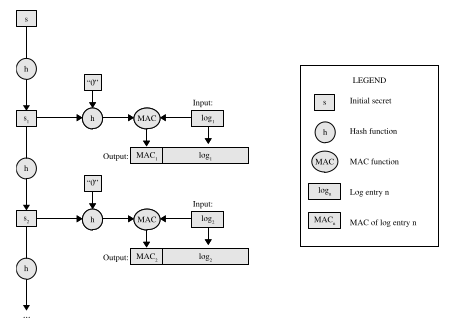
\includegraphics[scale=0.6]{imagenes/MAC.png}
\end{frame}

\begin{frame}
\frametitle{Verificación}
  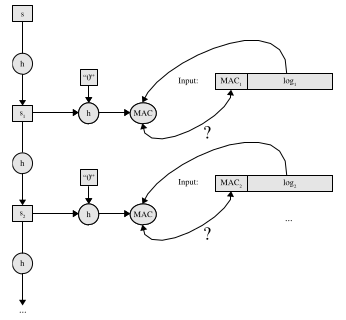
\includegraphics[scale=0.6]{imagenes/Verification.png}
\end{frame}

\begin{frame}
\frametitle{Cifrado}
  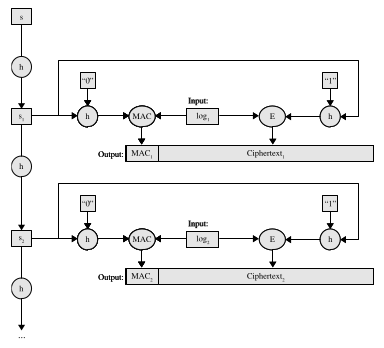
\includegraphics[scale=0.6]{imagenes/Cipher.png}
\end{frame}

\begin{frame}
\frametitle{Nuestra implementación}
\begin{itemize}
\item Utilizamos un secreto inicial, elegido por el administrador del equipo, para iniciar el servidor syslog.
Para cada log que se genere, se calcula su MAC y se guarda.
\item El propio administrador realizara la verificación de los logs aportando el secreto inicial.
\item Los registros de eventos se guardan en un ".log" de solo lectura para un usuario normal.
\item Cada verificación realiza el procedimiento descripto para todos los logs en el registro.
\end{itemize}
\end{frame}

\begin{frame}
\frametitle{Nuestra implementación}
Demo
\end{frame}

\begin{frame}
\frametitle{Alternativas}
Sistema de clave pública: consiste en generar claves privadas para firmar los logs, y claves publicas para verificarlos.
\begin{itemize}
\item Su principal ventaja es que no se necesita las claves privadas para realizar la verificación.
\end{itemize}
\end{frame}

\begin{frame}
\frametitle{Alternativas}
  \begin{figure}
    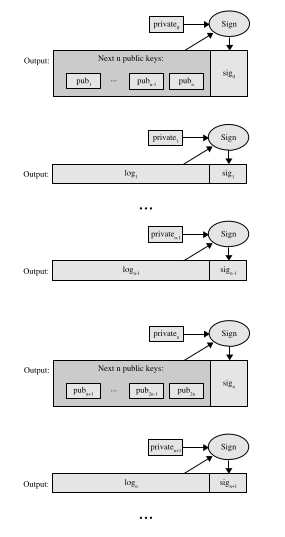
\includegraphics[scale=0.4]{imagenes/PublicKey.png}
  \end{figure}
\end{frame}

\begin{frame}
\frametitle{Sistema de clave pública}
\begin{figure}
  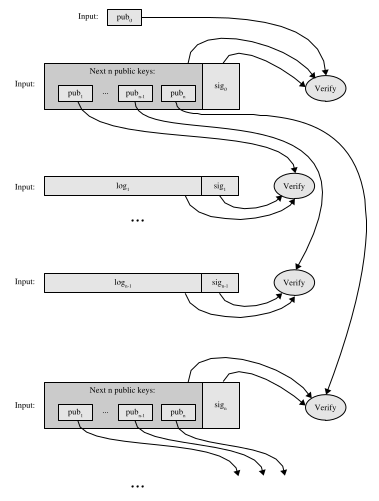
\includegraphics[scale=0.4]{imagenes/PublicKeyVerification.png}
\end{figure}
\end{frame}

\begin{frame}
\frametitle{Alternativas en la verificación}
\begin{itemize}
\item Existen dos alternativas a la hora de validar los logs:
\begin{itemize}
\item Validarlos todos(nuestra opción).
\item Validar solamente los que no fueron validados anteriormente(acumulativamente).
\end{itemize}
\end{itemize}
\end{frame}


% %%%         merkle trees
\begin{frame}
\frametitle{Investigaci\'on sobre \'arboles de Merkle o \'arboles de hash}
\begin{itemize}

\item Definici\'on: Es un \'arbol donde cada nodo contiene el hash de los hashes de sus hijos y las hojas contienen el hash del valor a proteger. En el nodo ra\'iz queda el hash que representa a todo el \'arbol, es decir que si alguno de los nodos modifica su hash invalidar\'a el hash de los nodos padres.
\item Fue patentado por Ralph Merkle en 1979, como m\'etodo de firmas digitales para robustecer el sistema criptogr\'afico presentado Diffie, Hellman y \'el dos a\~nos antes.

\end{itemize}
\end{frame}


\begin{frame}
\frametitle{Estructura de Hash Tree}

\begin{figure}
  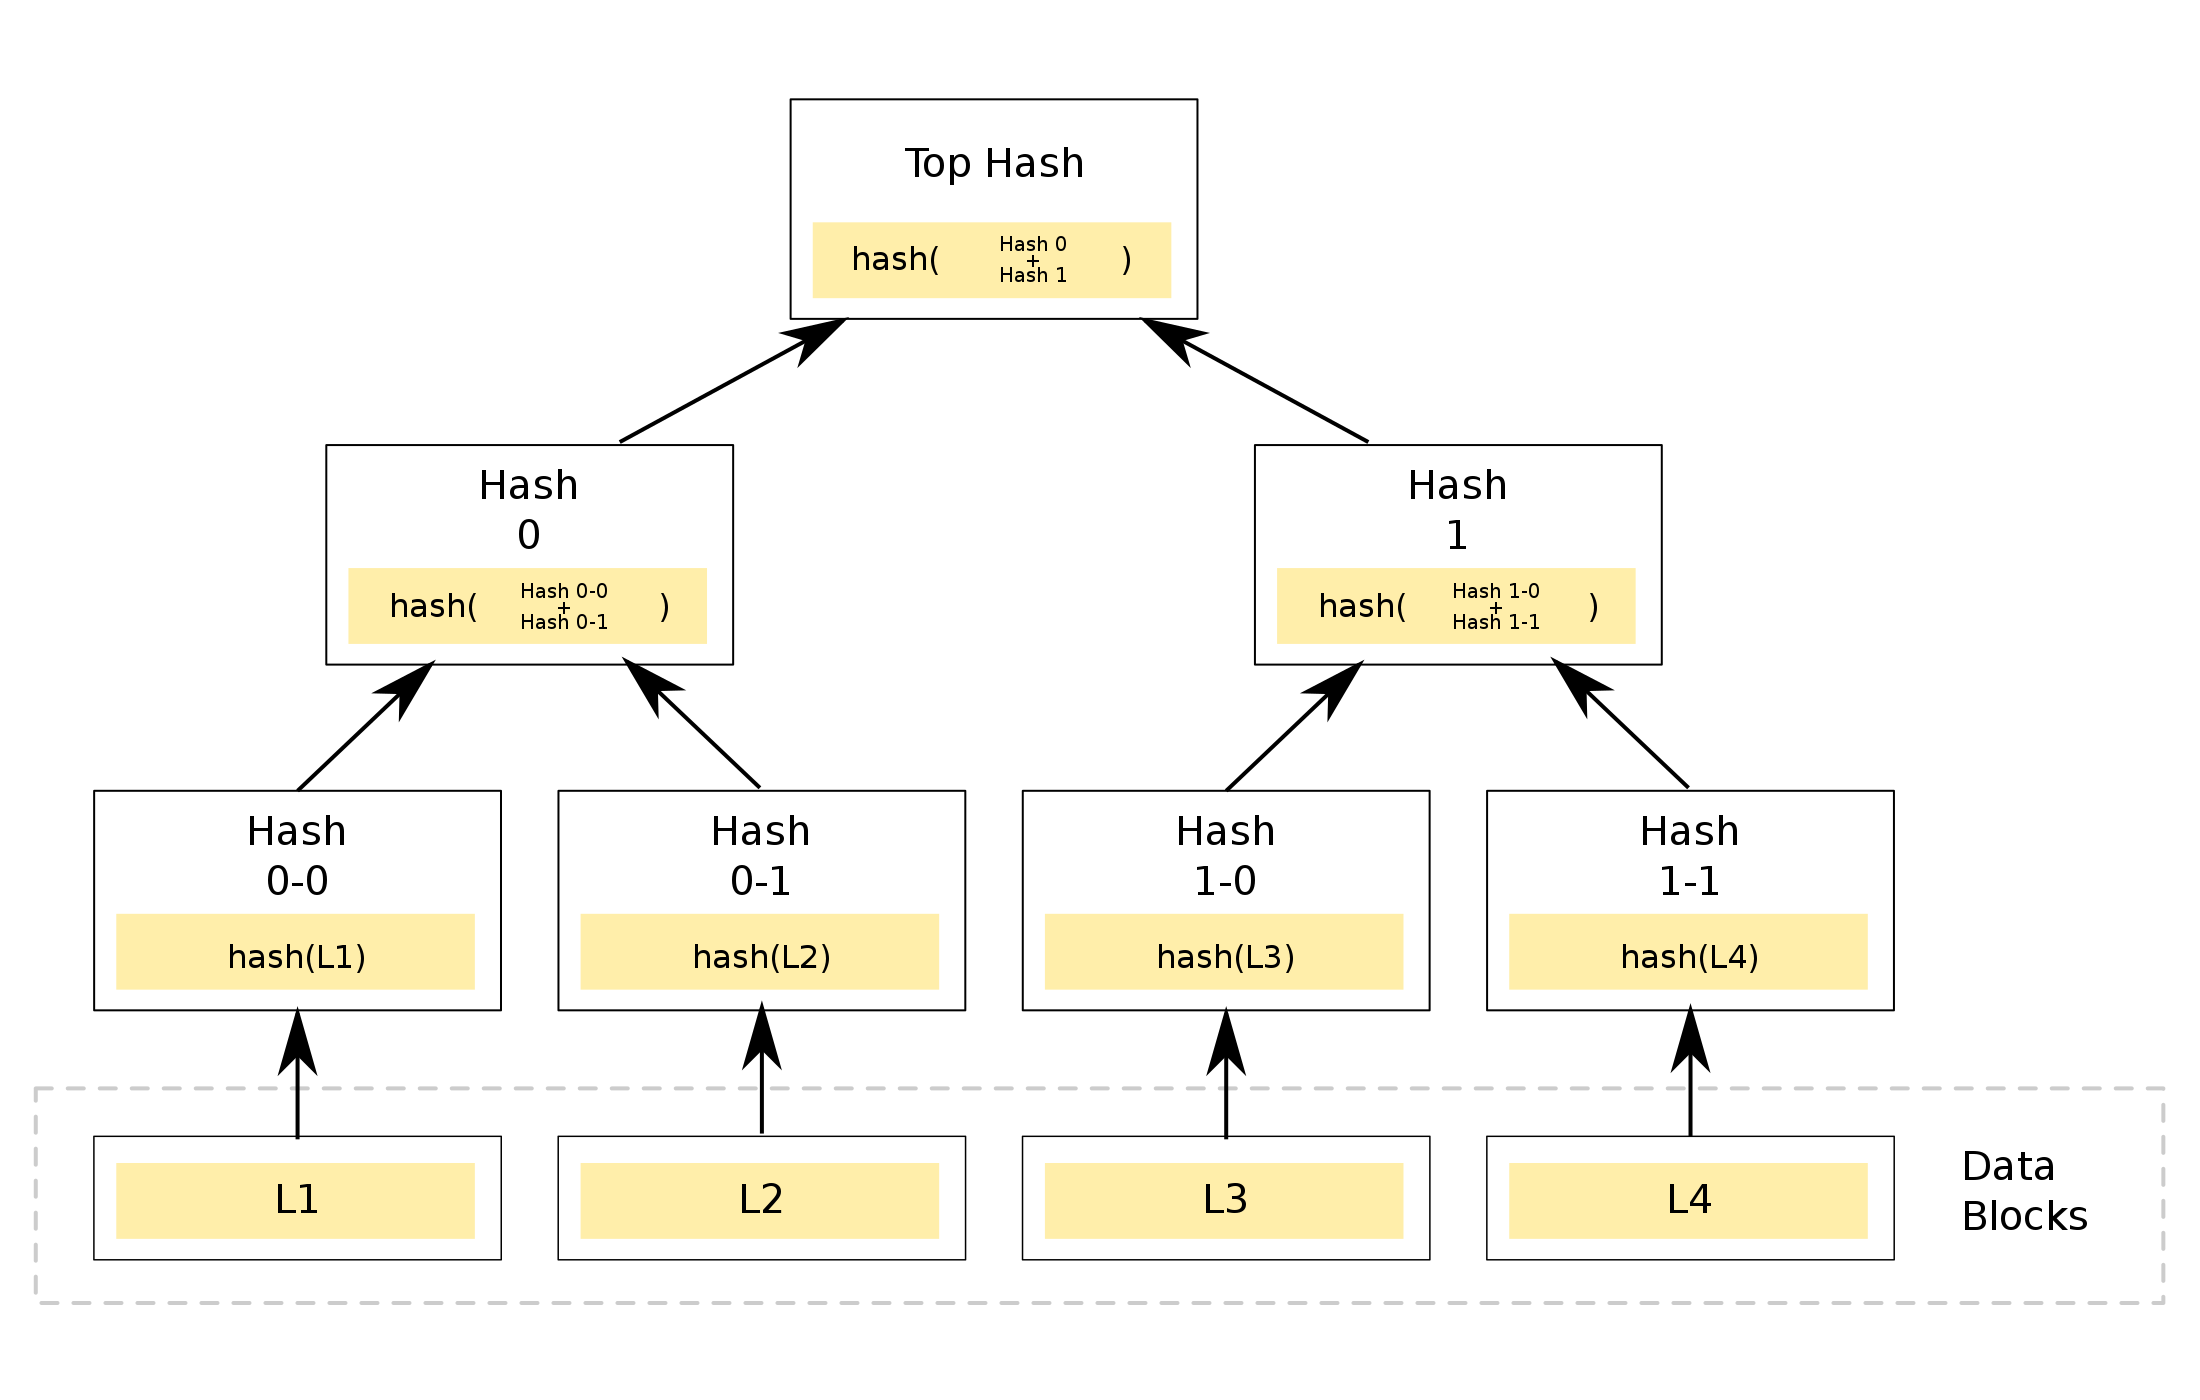
\includegraphics[width=\linewidth]{imagenes/hash_tree.png}
 % \caption{\'Arbol de Hash}
\end{figure}

\end{frame}


\begin{frame}
\frametitle{Principales caracter\'isticas}

\begin{itemize}

\item Merkle Audit Paths: Permite verificar si un bloque de datos protegido fue modificado con \'orden log(n), donde n es la cantidad de bloques de datos totales del \'arbol. As\'i s\'olo requiere calcular 2 * log2(n) hashes, correspondientes al camino desde la ra\'iz al valor a validar junto con los hijos de cada nodo del camino. La misma operaci\'on en listas de hash tiene orden n.

\item Merkle Consistency Proofs: Dada una lista de los primeros m bloques de datos permite verificar no se hayan borrado o agregado algunos, o modificado el \'orden entre ellos. Esta es una propiedad \'util para mejorar el syslog server.

\end{itemize}

\end{frame}




\begin{frame}
\frametitle{Usos}

\begin{itemize}

\item Certificate Transparency: Framework open source para el monitoreo y auditor\'ia de certificados digitales. A partir de un registro p\'ublico de la emisi\'on de los certificados los clientes pueden verificar su validez.

% imagenes de arquitectura y arbol, y m�s detalles

\item Redes peer-2-peer
\begin{itemize}

\item BitTorrent: Valida cada bloque descargado independientemente del archivo completo.
\item Bitcoin: Optimiza el tama\~no del blockchain guardando s\'olo el hash root de las transacciones cada bloque. Permite a los clientes escuchar de forma eficiente la publicaci\'on de transacciones asociadas a una billetera en particular.
\item Otros: Filesystems como IPFS, Sistemas de control de versiones como Git o Mercurial, bases de datos NoSQL como Cassandra o Dynamo.

% imagen del arbolitos del bloque de bitcoin

\end{itemize}

\end{itemize}


\end{frame}





\begin{frame}
\frametitle{Referencias}


\begin{itemize}

\item Wikipedia \(https://en.wikipedia.org/wiki/Merkle_tree\)
\item Certificate Transparency RFC \(https://tools.ietf.org/html/rfc6962\)
\item Forward Integrity For Secure Audit Logs de Mihir Bellare y Bennet S. Yee
\item Logcrypt: Forward Security and Public Verification for Secure Audit Logs de Jason E. Holt

\end{itemize}
\end{frame}


\end{document}
